\documentclass[11pt]{article}

\usepackage{listings}
\usepackage{amsmath,amsfonts,amssymb}
\usepackage{xcolor}
\usepackage{graphicx}
\usepackage{natbib}
\usepackage{float}

\title{CSE565M - Lab 2}
\author{Johnathan Dunker}
\date{\today}

\lstdefinestyle{HLSstyle}{
    backgroundcolor=\color{white}, % Choose the background color
    commentstyle=\color{gray}, % Comment color
    keywordstyle=\color{blue}, % Keyword color
    numberstyle=\tiny\color{gray}, % Line number style
    stringstyle=\color{red}, % String color
    basicstyle=\ttfamily, % Basic font style
    breakatwhitespace=true, % Break lines at whitespace
    breaklines=true, % Automatic line breaking
    captionpos=b, % Caption position
    numbers=left, % Line numbers on the left
    numbersep=5pt, % Distance of line numbers from code
    showspaces=false, % Show spaces
    showstringspaces=false % Don't show spaces in strings
}

\begin{document}
  \maketitle

    \section{Baseline Code}
      \subsection{fir11\_host.cpp}
      This code connects to the FPGA device and installs the kernel. It then sets up an output buffer, and reads an input file 'input.dat'. It goes over each input \texttt{data\_t}, defined in 'fir11\_kernel.h' as \texttt{int}, and passes it to the device. After that it waits for the device to finish then takes the output through the binary output and sends the data to the output file 'out.dat'. After it finishes through the input it compared the output with the contents of 'out.gold.fir11.dat'.

      \pagebreak[3]
      \subsection{Kernel}
        \begin{lstlisting}[style=HLSstyle, language=C++]
          extern "C" {
            void fir(data_t *y, data_t x) {
            #pragma HLS pipeline II = 1
              coef_t c[N] = {53, 0, -91, 0, 313, 500, 313, 0, -91, 0, 53};

              static data_t shift_reg[N];
              acc_t acc;
              int i;

              acc = 0;
              Shift_Accum_Loop:
                for(i = N - 1; i >= 0; i--) {
                  if (i == 0) {
                    acc += x * c[0];
                    shift_reg[0] = x;
                  } else {
                    shift_reg[i] = shift_reg[i - 1];
                    acc += shift_reg[i] * c[i];
                  }
                  *y = acc;
                }
            }
          }
        \end{lstlisting}
      \pagebreak[3]
      \subsection{Emulation}
      \begin{figure}[H]
        \centering
        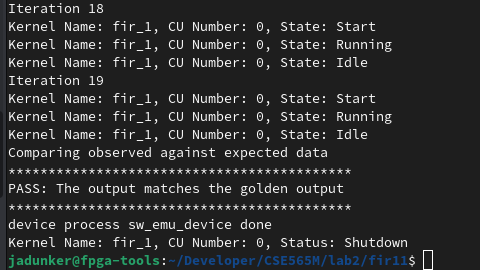
\includegraphics[width=0.8\textwidth]{baseline_sw_emu.png}
        \caption{Software Emulation Output}
        \label{fig:bl_sw_emu_out}
      \end{figure}
      \begin{figure}[H]
        \centering
        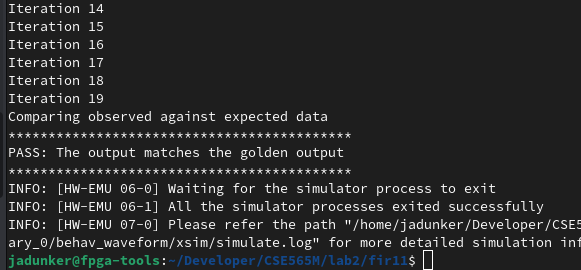
\includegraphics[width=0.8\textwidth]{baseline_hw_emu_2.png}
        \caption{Hardware Emulation Output}
        \label{fig:bl_hw_emu_out}
      \end{figure}
    
    \pagebreak[3]
    \section{Optimization}
      \begin{lstlisting}[style=HLSstyle, language=C++]
        extern "C" {
          void fir(data_t *y, data_t x) {
          #pragma HLS pipeline II = 1
            coef_t c[N] = {53, 0, -91, 0, 313, 500, 313, 0, -91, 0, 53};

            static data_t shift_reg[N];
            #pragma HLS ARRAY_PARTITION variable = shift_reg complete dim = 0
            acc_t acc;
            int i;

            acc = 0;
            TDL:
              for(i = N - 1; i > 0; i--)
              {
                #pragma HLS PIPELINE II = 1
                shift_reg[i] = shift_reg[i-1];
              }
              shift_reg[0] = x;
            MAC:
              for(i = N - 1; i >= 0; i--) {
                #pragma HLS PIPELINE II = 1
                acc += shift_reg[i] * c[i];
              }
            *y = acc;
          }
        }
      \end{lstlisting}
      \pagebreak[3]
      \subsection{Emulation}
      \begin{figure}[H]
        \centering
        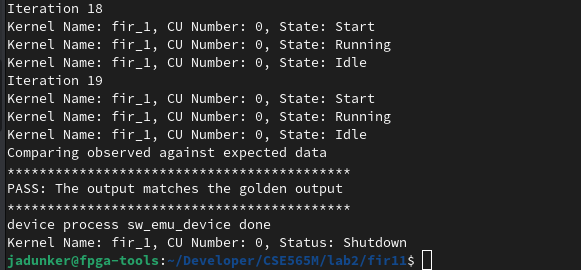
\includegraphics[width=0.8\textwidth]{opt_sw_emu.png}
        \caption{Software Emulation Output}
        \label{fig:opt_sw_emu_out}
      \end{figure}
      \begin{figure}[H]
        \centering
        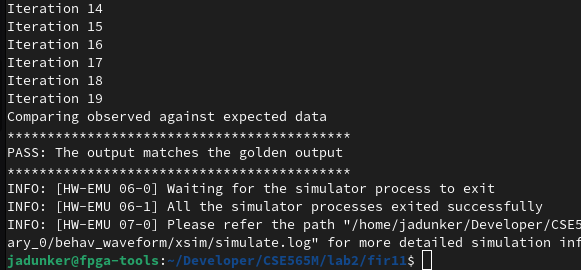
\includegraphics[width=0.8\textwidth]{opt_hw_emu.png}
        \caption{Hardware Emulation Output}
        \label{fig:opt_hw_emu_out}
      \end{figure}
    \section{Vitis GUI}
      \begin{figure}[H]
        \centering
        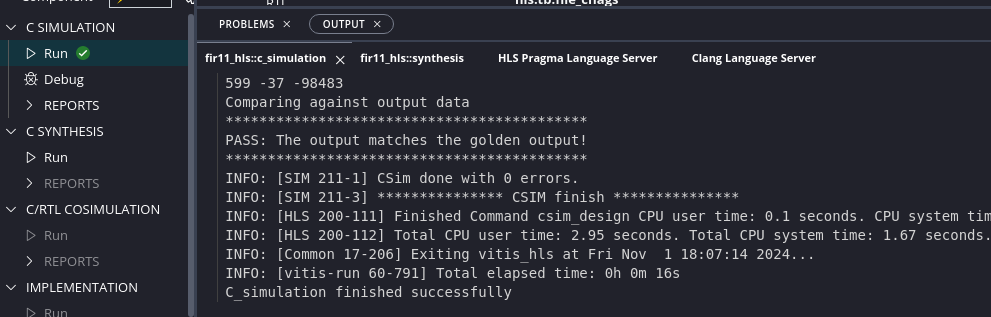
\includegraphics[width=0.8\textwidth]{vitis_c_sim_2.png}
        \caption{Vitis C Simulation}
        \label{fig:vitis_c_sim}
      \end{figure}
      \begin{figure}[H]
        \centering
        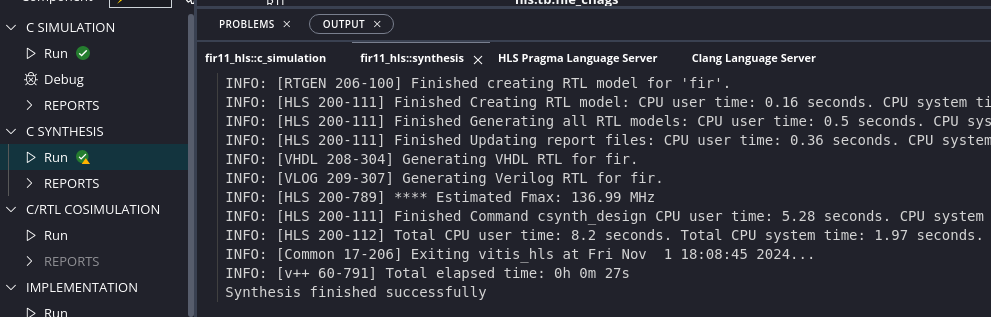
\includegraphics[width=0.8\textwidth]{vitis_c_syn.png}
        \caption{Vitis C Synthesis}
        \label{fig:vitis_c_syn}
      \end{figure}

      The most interesting report I found in the vitis GUI was the the block schedule. It showed
      when each logical portion of the kernel would execute. Personally, I found it humorous that
      communication with the FPGA was 8x longer than the kernel itself.

      \begin{figure}[H]
        \centering
        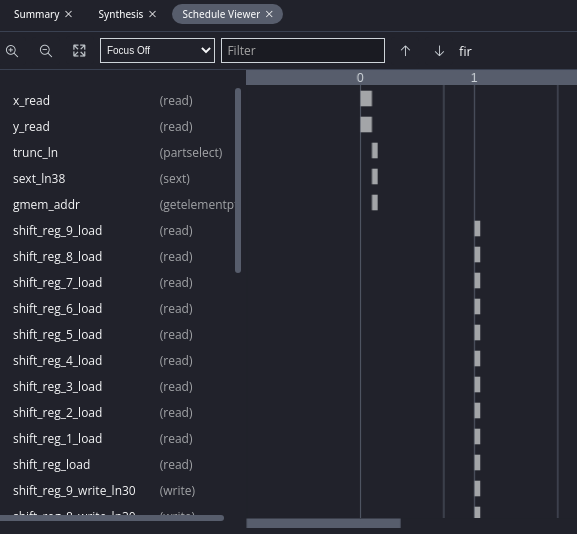
\includegraphics[width=0.8\textwidth]{vitis_sched_1.png}
        \hfill
        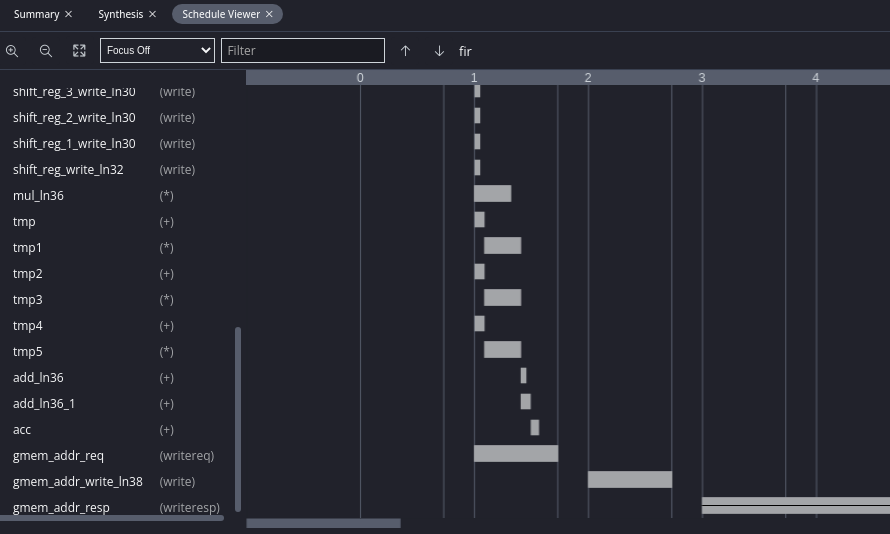
\includegraphics[width=0.8\textwidth]{vitis_sched_2.png}
        \caption{Logic Block Schedule}
        \label{fig:vitis_sched_2}
      \end{figure}

      I also found the Quality of Results report interesting. It estimated the timing of the kernel along
      with describing the pipeline's size latency, initiation interval and the bram and dsp usage.

      \begin{figure}[H]
        \centering
        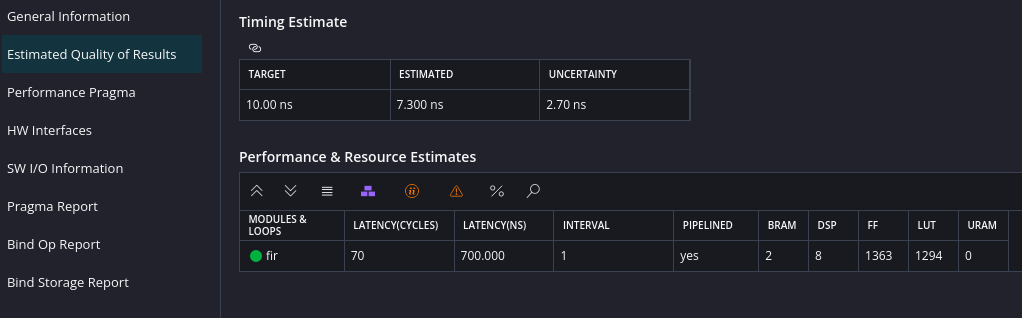
\includegraphics[width=0.8\textwidth]{vitis_QoR.png}
        \caption{Estimated Quality of Results Report}
        \label{fig:vitis_QoR}
      \end{figure}
\end{document}